% =============================================================================
% COPYRIGHT AND DISCLAIMER
% =============================================================================
% This file is provided as a convenience template for competition participants.
% By using it, you accept full responsibility for compliance with all applicable
% copyright, licensing, and usage rules of the Association for Computing
% Machinery (ACM) and of any LaTeX packages you load (including, without
% limitation, the "acmart" document class and related ACM materials).
%
% Consult ACM's official publication, template, and copyright policies before
% using this setup for any purpose other than this competition. Do not assume
% that this template may be reused, redistributed, or submitted elsewhere
% without independently verifying ACM's current rules.
%
% Use of the "acmart" class, the "sigconf" option, or ACM-style formatting in
% this template does NOT mean that this report, this competition, its organizers,
% or any resulting PDF is sponsored, endorsed, affiliated with, or published by
% ACM. ACM trademarks and branding remain the property of ACM.
%
% Template packages live in preamble.tex.
% Citations live in main.bib. Edit this file with your paper content.
% =============================================================================

\documentclass[sigconf]{acmart}
% =============================================================================
% Template setup — participants normally do not edit this file.
% Author content belongs in main.tex; citations belong in main.bib.
% \documentclass lives in main.tex so Overleaf does not treat this file as root.
% =============================================================================

% --- Competition / non-ACM-submission friendly rights metadata -------------
\setcopyright{none}
\settopmatter{printacmref=false}
\acmConference[Kaggle Competition]{Filament Segmentation Challenge}{2026}{\href{https://www.kaggle.com/competitions/filament-segmentation-2026}{kaggle.com/competitions/filament-segmentation-2026}}
\acmBooktitle{Competition Report}
\acmDOI{}
\acmISBN{}

% --- Author guidance text --------------------------------------------------
% \guide{...} is gray italic while \guideStyletrue; omitted from the PDF if false.
% Flip the switch in main.tex after % =============================================================================
% Template setup — participants normally do not edit this file.
% Author content belongs in main.tex; citations belong in main.bib.
% \documentclass lives in main.tex so Overleaf does not treat this file as root.
% =============================================================================

% --- Competition / non-ACM-submission friendly rights metadata -------------
\setcopyright{none}
\settopmatter{printacmref=false}
\acmConference[Kaggle Competition]{Filament Segmentation Challenge}{2026}{\href{https://www.kaggle.com/competitions/filament-segmentation-2026}{kaggle.com/competitions/filament-segmentation-2026}}
\acmBooktitle{Competition Report}
\acmDOI{}
\acmISBN{}

% --- Author guidance text --------------------------------------------------
% \guide{...} is gray italic while \guideStyletrue; omitted from the PDF if false.
% Flip the switch in main.tex after % =============================================================================
% Template setup — participants normally do not edit this file.
% Author content belongs in main.tex; citations belong in main.bib.
% \documentclass lives in main.tex so Overleaf does not treat this file as root.
% =============================================================================

% --- Competition / non-ACM-submission friendly rights metadata -------------
\setcopyright{none}
\settopmatter{printacmref=false}
\acmConference[Kaggle Competition]{Filament Segmentation Challenge}{2026}{\href{https://www.kaggle.com/competitions/filament-segmentation-2026}{kaggle.com/competitions/filament-segmentation-2026}}
\acmBooktitle{Competition Report}
\acmDOI{}
\acmISBN{}

% --- Author guidance text --------------------------------------------------
% \guide{...} is gray italic while \guideStyletrue; omitted from the PDF if false.
% Flip the switch in main.tex after \input{preamble}.
%
% Do not use \guide{...} for \email{...}.
\usepackage{xcolor}
\newif\ifguideStyle
\guideStyletrue
\newcommand{\guide}[1]{%
  \ifguideStyle
    {\color{gray!65}\itshape #1}%
  \fi
}

% --- Math ------------------------------------------------------------------
% Do NOT load amssymb (or amsfonts): acmart already loads newtxmath, which
% defines the same symbols (e.g. \Bbbk) and causes a conflict on Overleaf.
% amsmath is already provided by acmart; mathtools extends it.
\usepackage{mathtools}

% --- Figures ---------------------------------------------------------------
% graphicx is already loaded by acmart
\usepackage{subcaption}

% --- Tables ----------------------------------------------------------------
% booktabs is already loaded by acmart
\usepackage{tabularx}
\usepackage{multirow}

% --- Bibliography style is set in main.tex (ACM-Reference-Format) ----------

% --- Pipeline diagram (TikZ) -------------------------------------------------
\usepackage{tikz}
\usetikzlibrary{arrows.meta, positioning, fit}
.
%
% Do not use \guide{...} for \email{...}.
\usepackage{xcolor}
\newif\ifguideStyle
\guideStyletrue
\newcommand{\guide}[1]{%
  \ifguideStyle
    {\color{gray!65}\itshape #1}%
  \fi
}

% --- Math ------------------------------------------------------------------
% Do NOT load amssymb (or amsfonts): acmart already loads newtxmath, which
% defines the same symbols (e.g. \Bbbk) and causes a conflict on Overleaf.
% amsmath is already provided by acmart; mathtools extends it.
\usepackage{mathtools}

% --- Figures ---------------------------------------------------------------
% graphicx is already loaded by acmart
\usepackage{subcaption}

% --- Tables ----------------------------------------------------------------
% booktabs is already loaded by acmart
\usepackage{tabularx}
\usepackage{multirow}

% --- Bibliography style is set in main.tex (ACM-Reference-Format) ----------

% --- Pipeline diagram (TikZ) -------------------------------------------------
\usepackage{tikz}
\usetikzlibrary{arrows.meta, positioning, fit}
.
%
% Do not use \guide{...} for \email{...}.
\usepackage{xcolor}
\newif\ifguideStyle
\guideStyletrue
\newcommand{\guide}[1]{%
  \ifguideStyle
    {\color{gray!65}\itshape #1}%
  \fi
}

% --- Math ------------------------------------------------------------------
% Do NOT load amssymb (or amsfonts): acmart already loads newtxmath, which
% defines the same symbols (e.g. \Bbbk) and causes a conflict on Overleaf.
% amsmath is already provided by acmart; mathtools extends it.
\usepackage{mathtools}

% --- Figures ---------------------------------------------------------------
% graphicx is already loaded by acmart
\usepackage{subcaption}

% --- Tables ----------------------------------------------------------------
% booktabs is already loaded by acmart
\usepackage{tabularx}
\usepackage{multirow}

% --- Bibliography style is set in main.tex (ACM-Reference-Format) ----------

% --- Pipeline diagram (TikZ) -------------------------------------------------
\usepackage{tikz}
\usetikzlibrary{arrows.meta, positioning, fit}


% Guide styling: no longer needed once the author/affiliation fields below are
% filled in; guide mode is now off. The title is plain (black) text rather than
% \guide{}-wrapped: acmart derives PDF metadata (pdftitle) from \title{}, and
% wrapping it in color/italic-switching macros corrupts that metadata field.
% A short-title form is passed via \title[short]{full} so the running header on
% pages 2+ does not collide with the venue line (reviewer feedback, 2026-08-30).
\guideStylefalse

\begin{document}

\title[Detect, Refine, Resolve]{Detect, Refine, Resolve: An Edge-Attention-Inspired Boundary Refiner for Solar Filament Instance Segmentation}
\subtitle{A Solution to the Solar Filament Segmentation Challenge 2026} % DO NOT CHANGE

\author{Shingo Hara}
\affiliation{%
  \institution{ER Systems, Ltd.}
  \city{Kanagawa}
  \country{Japan}
}
\email{shingo257@gmail.com}
\renewcommand{\shortauthors}{Hara}

\begin{abstract}
    This report describes our solution to the Solar Filament Segmentation Challenge~2026, a Kaggle competition on segmenting solar filaments in GONG H-$\alpha$ observations. Our pipeline detects candidates with a YOLO11-seg instance detector, refines their boundaries with a crop-level U-Net, and resolves overlaps into a disjoint instance set, with design decisions evaluated under leak-free 3-fold cross-validation and an observation-cluster bootstrap --- a protocol that rejected five plausible improvements whose single-fold gains did not replicate. One further change --- an EdgeAttNet-inspired~\cite{edgeattnet2025} edge-guided self-attention block at the refiner's bottleneck --- initially passed this protocol ($\Delta$PQ$=+0.0028$, 95\% CI $[0.00091,0.00476]$, all folds agreeing) and moved the public leaderboard score from $0.37$ to $0.39$. A follow-up matched-parameter ablation (all folds, two seeds) refines this picture: bottleneck attention capacity, with or without the edge prior, tends to help (positive in two folds, neutral in the third), but the edge prior itself shows no consistent benefit over plain attention. Our main finding is this refinement: our acceptance criterion could not separate a general capacity effect from the specific edge-prior mechanism we set out to validate.
\end{abstract}

\maketitle

% ==================================== %
%              INTRODUCTION            %
% ==================================== %
\section{Introduction}
    This report describes our submitted solution to the Solar Filament Segmentation Challenge~2026~\cite{filament-segmentation-2026}, organized by the Earth-Space AI Research (ESAIR) Lab and scored against the MAGFiLO dataset~\cite{ahmadzadeh2024dataset}. Our approach treats the task as instance segmentation: detect each filament as a separate object, refine its boundary, and reconcile overlapping candidates into a single non-overlapping prediction set. Section~\ref{sec:methodology} describes the pipeline; Section~\ref{sec:evaluation} reports our evaluation protocol, results, and an honest account of what we tried that did \emph{not} work.

% ==================================== %
%              METHODOLOGY             %
% ==================================== %
\section{Methodology}\label{sec:methodology}

\begin{figure*}[t]
    \centering
    \begin{tikzpicture}[
        node distance=4.5mm,
        box/.style={draw, rounded corners, minimum height=0.92cm, minimum width=2.35cm, align=center, font=\footnotesize, fill=gray!8},
        arr/.style={-{Latex[length=2mm]}, thick}
    ]
        \node[box] (raw) {H-$\alpha$\\FITS/JPEG};
        \node[box, right=of raw] (prep) {Preprocess\\background flatten +\\CLAHE/black-hat};
        \node[box, right=of prep] (yolo) {YOLO11-seg\\detector\\(per-fold)};
        \node[box, right=of yolo] (refine) {Edge-attention\\U-Net refiner\\(320px crops)};
        \node[box, right=of refine] (own) {Ownership\\resolution\\(IoU containment +\\greedy exclusivity)};
        \node[box, right=of own, fill=gray!18] (final) {Final disjoint\\instance masks};
        \draw[arr] (raw) -- (prep);
        \draw[arr] (prep) -- (yolo);
        \draw[arr] (yolo) -- node[above, font=\scriptsize]{proposals + scores} (refine);
        \draw[arr] (refine) -- node[above, font=\scriptsize]{shrunk masks} (own);
        \draw[arr] (own) -- (final);
    \end{tikzpicture}
    \caption{End-to-end inference pipeline. Training uses leak-free 3-fold cross-validation (Section~\ref{sec:cv}); the submitted model uses a single detector fold plus a refiner fine-tuned on all folds.}
    \label{fig:pipeline}
\end{figure*}

\subsection{Preprocessing}
    Raw GONG H-$\alpha$ observations are $2048\times2048$ single-channel intensity images. Each image is encoded into a 3-channel input so that the detector backbone can reuse standard RGB-pretrained weights while still operating on physically meaningful contrast bands: channel 1 is a percentile-clipped copy of the raw intensity; channel 2 divides the image by a large-kernel Gaussian estimate of the background (flattening limb darkening and the radial illumination gradient) followed by CLAHE; channel 3 is a black-hat morphological transform of channel 2, which isolates dark, thin, filament-scale detail. (A separate histogram-matching step is used only for the rejected pseudo-labeling experiment, not the main pipeline.)

\subsection{Detection}
    Filament candidates are generated by \textbf{YOLO11m-seg}~\cite{yolo11}, an anchor-free, NMS-based instance segmentation network, trained and run at $1280\times1280$ with a single foreground class. We trained one detector per fold (Section~\ref{sec:cv}) for up to 70 epochs (patience 14), batch size 4, seed $3407+\text{fold}$, \texttt{deterministic=True}. AdamW ($\text{lr}_0{=}7{\times}10^{-4}$, $\text{lr}_f{=}0.05$, weight decay $5{\times}10^{-4}$, 3-epoch warmup); geometric augmentation (rotation $\pm180^\circ$, translate $0.04$, scale $0.25$, flips $p{=}0.5$); mosaic $0.20$ (off for the final 10 epochs); no hue/saturation jitter (meaningless for this encoding); value jitter $0.18$; mask downsample 2. Inference uses confidence $0.26$, NMS IoU $0.55$; the full machine-readable call is in \texttt{scratch/}. We chose YOLO11-seg over RF-DETR-Seg~\cite{rfdetr2025} after a same-split comparison: RF-DETR-Seg's raw PQ trailed by $-0.057$. Not a matched-hyperparameter comparison, so this rules out a drop-in replacement, not the architecture family.

\subsection{Boundary Refinement}\label{sec:refiner}
    Raw detector masks are accurate in extent but imprecise at the pixel boundary, which is exactly where the official metric is least forgiving (Section~\ref{sec:evaluation-strategy}). We refine each candidate independently: a square crop is taken around the candidate ($1.65\times$ its bounding box, minimum side 96px, $320\times320$px after resizing), passed through a U-Net refiner, and the resulting probability map is thresholded (0.45) and intersected with the original candidate mask (\emph{shrink} refinement — the refiner may only remove pixels, not add them outside the detector's proposal).

    \textbf{Training data.} Positive crops are generated one per ground-truth instance per annotator (a 3-annotator image contributes up to $3\times$ the crops of a single-annotator image), centered and scaled from that instance's box with the same $1.65\times$-context rule as inference; no hard-negative crops. Augmentation: random $90^\circ$ rotations, flips, mild gamma jitter on the first two channels.

    \textbf{Optimization.} We minimize $0.35\cdot\text{BCE} + 0.65\cdot\text{soft-Dice} + 0.15\cdot\text{boundary-}L_1$, where the boundary term compares a morphological-gradient (dilation$-$erosion, kernel 5) map of prediction and target. AdamW (weight decay $10^{-4}$), lr $2{\times}10^{-4}$ cosine-annealed, AMP, batch size 8. Per-fold refiners train 14 epochs (seed 3407), keeping the best validation crop-Dice checkpoint. The submitted refiner is fine-tuned from the fold-0 checkpoint on all 707 images for 5 epochs at $0.35\times$ the base lr (Section~\ref{sec:cv}); with no held-out data, we keep the final-epoch weights.

    Our refiner, \texttt{MediSegEdgeAttUNet}, extends this U-Net~\cite{ronneberger2015unet} with a single \textbf{edge-guided multi-head self-attention} (EG-MHSA) block at the bottleneck (8 heads), \emph{inspired by} EdgeAttNet~\cite{edgeattnet2025}: a $3{\times}3$ conv on the crop yields an edge prior, projected and added to the attention query and key (not value), before residual and layer norm. EdgeAttNet's public code lacks a usable implementation of this module, so we could not validate against it, and our design deviates: EdgeAttNet stacks \emph{two} 4-head blocks and \emph{drops} positional encodings, shrinking to 22.7M params (vs.\ its 31.0M baseline), while ours \emph{adds} 4.2M (35.2M vs.\ 31.0M) --- matching the parameter count of EdgeAttNet's own ``U-Net + MHSA, no positional encoding'' ablation almost exactly. We therefore call it edge-attention-inspired, not a reproduction; Section~\ref{sec:evaluation} revisits what this coincidence implies.

\subsection{Instance Resolution}
    Refined candidates can still overlap (two proposals covering the same physical filament, or a small proposal nested inside a larger one). We remove near-duplicates whose intersection covers $\geq\!90\%$ of the smaller candidate's area, then greedily assign remaining pixels to candidates in ascending order of area (small, precise candidates claim their pixels before large ones), discarding any candidate left with fewer than 20px. This ordering outperformed confidence-first and area-descending orderings by $0.012$--$0.015$~PQ in a final three-fold audit (Section~\ref{sec:strengths}).

\subsection{Cross-Validation and Final Model}\label{sec:cv}
    The competition provides 707 training images, each annotated by one or more experts (8{,}199 instance annotations; all annotators used as independent targets). We group by unique observation filename --- preventing fold-boundary leakage by construction --- and partition into three folds (236/236/235) with a stratified $k$-fold splitter (seed 3407) on quintiles of each image's reference-annotator instance count. One detector and one refiner are trained per fold. For the final submission we select the best-PQ detector fold and fine-tune the refiner on \emph{all} 707 images (warm-started, 5 epochs, $0.35\times$ base lr), keeping cross-validated model selection intact.

\begin{figure*}[t]
    \centering
    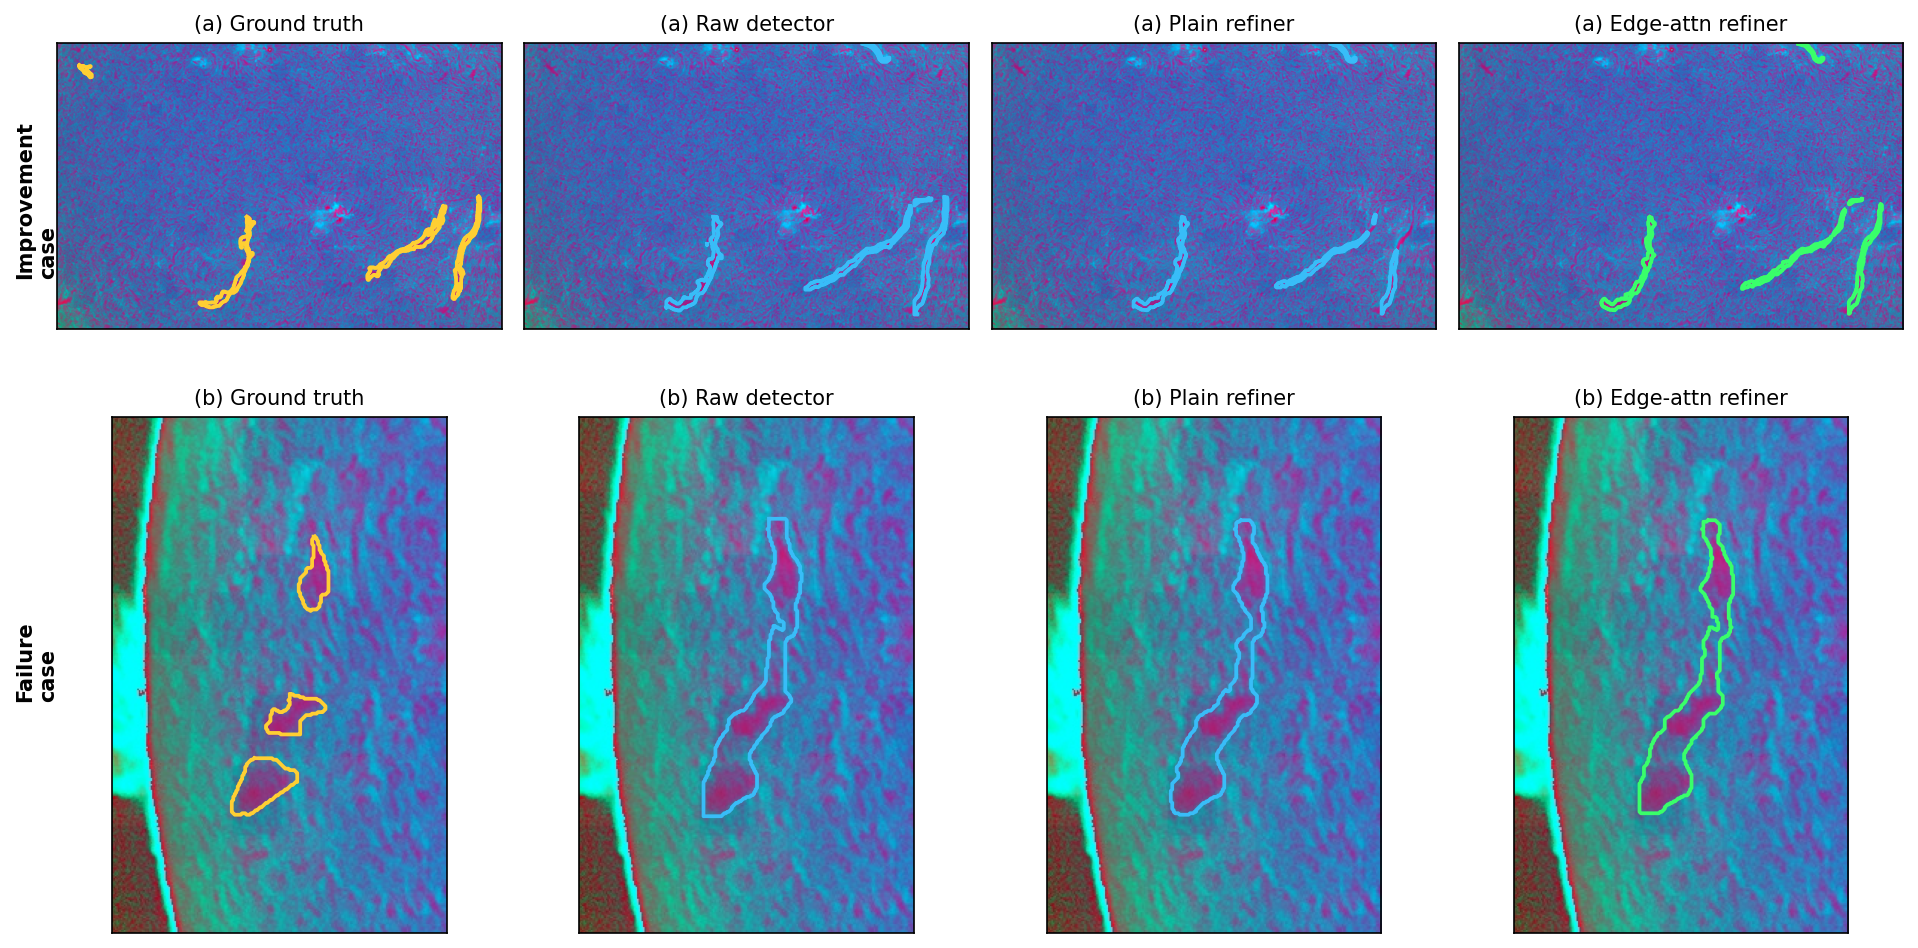
\includegraphics[width=0.60\linewidth]{figures/qualitative_comparison.png}
    \caption{Ground truth vs.\ raw detector vs.\ plain vs.\ edge-attention refiner, fold-0 OOF. \textbf{(a)}: three filaments where edge attention recovers more true extent than plain (IoU $0.36{\rightarrow}0.59$, $0.43{\rightarrow}0.62$, $0.39{\rightarrow}0.56$). \textbf{(b)}: the detector merges two ground-truth instances into one candidate and misses a third; all refiners inherit this detector-level failure. From the original single-seed run; the ablation did not reproduce (a).}
    \label{fig:example}
\end{figure*}

% ==================================== %
%              EVALUATION              %
% ==================================== %
\section{Evaluation}\label{sec:evaluation}

\subsection{Evaluation Strategy}\label{sec:evaluation-strategy}
    The competition's official metric is Panoptic Quality (PQ), following the definition of Kirillov et al.~\cite{kirillov2019panoptic} but scored by the competition's own reference implementation~\cite{selfeval2026}, which we replicated locally against that notebook's test cases. Unlike the original PQ formulation's one-to-one Hungarian matching, the competition scorer counts \emph{every} prediction-ground-truth pair with IoU above $0.5$ as a true positive (i.e.\ both sides can be matched multiply), so
    \[
        \mathrm{PQ} = \frac{\sum_{(p,g)\in TP}\mathrm{IoU}(p,g)}{|TP| + 0.5|FP| + 0.5|FN|}.
    \]
    A prediction with IoU just under 0.5 scores zero \emph{and} incurs a false-positive/false-negative penalty, so near-miss boundary quality dominates the score far more than raw detection recall. Matching is done per (annotator, image) pair and micro-averaged, not averaged per-image.

    Because annotators disagree, we measured a reference-annotation agreement baseline: scoring one expert's annotations as the ``prediction'' against every other expert on the same image, under the identical official rule, gives PQ$=0.3398$ (multi-annotator images only, $n{=}296$; an earlier version trivially included self-matches, inflating it to $0.76$ --- corrected). Not a hard ceiling (ours scores above it); it is a benchmark for labeling-task reproducibility.

    All model-selection decisions use the leak-free 3-fold cross-validation of Section~\ref{sec:cv}. To avoid a failure mode we caught twice --- a change that improves one fold but does not replicate --- we additionally compute an observation-cluster bootstrap~\cite{efron1993bootstrap} (2000 resamples, PQ as ratio-of-sums) and accept a change only when (a)~its sign agrees across all folds and (b)~its pooled 95\% CI excludes zero ((a) alone is weak: $2{\times}0.5^3{=}0.25$ under a symmetric null). The pooled interval is reported for the one accepted change; rejected changes are summarized in Section~\ref{sec:strengths}. We apply no multiple-comparisons correction across the ${\sim}$dozen ideas evaluated on the same 707 OOF images, so nominal intervals are optimistic; we flag this rather than adjust post hoc.

\subsection{Results}\label{sec:results-discussion}
    Table~\ref{tab:results} summarizes our out-of-fold (OOF) results under this protocol, and the corresponding public leaderboard scores where we submitted a matching variant. Note that our OOF PQ ($0.4426$, plain refiner over all 707 images) exceeds the $0.3398$ reference-annotation agreement baseline of Section~\ref{sec:evaluation-strategy}: this is not evidence the model is more \emph{correct} than a human annotator, but it is consistent with the model, trained on pooled labels of several annotators, converging toward a consensus boundary that matches any single held-out annotator more often than two annotators match each other.

    \begin{table}[t]
    \centering
    \small
    \begin{tabularx}{\linewidth}{@{}X r r r@{}}
    \toprule
    Configuration & OOF PQ & SQ / RQ & Public LB \\
    \midrule
    Raw detector only & $0.3937$ & $0.652$ / $0.604$ & --- \\
    \quad + refiner + resolution & $0.4426$ & $0.678$ / $0.653$ & $0.37$ \\
    \quad\quad + edge-attention refiner & $0.4454^{\dagger}$ & ---$^{\dagger}$ & $\mathbf{0.39}$ \\
    \midrule
    \multicolumn{4}{@{}l}{\emph{Ablations submitted for direct comparison:}}\\
    3-fold ensemble (standard refiner) & --- & --- & $0.37$ \\
    3-fold ensemble (edge-attention) & --- & --- & $0.38$ \\
    \midrule
    \multicolumn{4}{@{}l}{\emph{Matched-param.\ ablation, all 3 folds, 2 seeds each$^{\ddagger}$:}}\\
    Plain U-Net (31.04M params) & $0.4418$ & $0.678$ / $0.651$ & --- \\
    + plain MHSA, no edge prior (35.24M) & $0.4432$ & $0.681$ / $0.651$ & --- \\
    + edge-guided MHSA (35.24M) & $0.4429$ & $0.678$ / $0.653$ & --- \\
    \bottomrule
    \end{tabularx}
    \caption{PQ, SQ, RQ leak-free; first two blocks over all 707 images (raw detector TP/FP/FN $=4765/2824/3434$; $+$refiner$+$resolution $5082/2286/3117$). $^{\dagger}$The single-seed $0.4454$ ($\Delta=+0.0028$, 95\% CI $[0.00091,0.00476]$) was originally accepted and submitted (LB $0.39$); the follow-up ablation did not reproduce it. $^{\ddagger}$Seeds 3407/8407, per-seed values in \texttt{output/ablation/}. Public LB is Kaggle's public score; the private leaderboard (undisclosed until competition end) determines final ranking.}
    \label{tab:results}
    \end{table}

    The edge-attention refiner's original per-fold deltas over the plain U-Net were $+0.0062$/$+0.0009$/$+0.0012$ (folds 0/1/2), sign-consistent with a pooled bootstrap CI $[0.00091,0.00476]$ excluding zero, so under our criterion we accepted and submitted it. The ablation below shows that acceptance attributed the effect to the wrong mechanism.

    \label{sec:matched-param-ablation}\textbf{Matched-parameter ablation.} To isolate whether the edge prior itself drives the effect, or whether added bottleneck attention capacity suffices, we ran seeds 3407/8407 on all three folds for three refiner variants: plain U-Net (31.04M params), bottleneck MHSA with no edge prior, and the edge-attention refiner (both 35.24M, differing by only ${\sim}2{,}100$ params --- these two \emph{are} matched). Per-fold mean OOF PQ (base/plain-attn/edge-attn): fold~0 $0.4414/0.4413/0.4405$; fold~1 $0.4405/0.4426/0.4417$; fold~2 $0.4434/0.4458/0.4464$. Attention-minus-base is positive in folds 1--2 for both attention variants; edge-minus-plain-attention is at or below zero in two folds --- no fold shows the edge prior clearly beating plain attention (\texttt{output/ablation/}).

    The originally reported improvement (LB $0.39$ vs.\ $0.37$ plain) does not survive this check and may reflect leaderboard noise; the re-introduced 3-fold ensemble scored $0.38$. An expected-IoU scorer reported $+0.0034$ exploratory OOF gain but $0.37$ publicly; its upstream caches were not nested by outer fold, so it is neither unbiased OOF nor adoption evidence.

    A $\chi^2$ test over file-name metadata found no train/test shift in observation year or site to explain the ${\sim}0.06$ OOF-to-LB gap ($p{=}0.42/0.94$).

    \textbf{Submission evidence.} Plain-MHSA fold-2 and edge-attention fold-2 checkpoint variants scored $0.39$ publicly (best-match IoU $0.94$/$0.93$ vs.\ production), motivating production plus plain-MHSA as architecture-diverse final candidates (Kaggle T4 inference ${\sim}1.1$\,s/image). These runs predate a verified input--code--model--split--output manifest, and an alternate split copy differs on 489/707 observations; the weights dataset therefore ships the consumed fold file \texttt{grouped\_folds\_train.csv} (SHA-256 \texttt{febb3f67\ldots}, OOF-cache agreement) alongside the pinned registry copy (\texttt{24367120\ldots}) --- retraining must use the former. The reproduction notebook regenerates both selected submissions byte-identically in a clean Kaggle environment. Other participants' provenance and scores were not independently verified.

\subsection{Strengths and Weaknesses}\label{sec:strengths}
    \textbf{Strengths.} Five candidates were rejected under confirmation across independent folds, bootstrap intervals, or matched public-LB comparison (mask fusion, threshold retuning, refiner retraining, pseudo-labeling, 3-fold ensembling). The one accepted change --- edge-guided attention --- did not survive the matched-parameter, multi-seed check (Section~\ref{sec:results-discussion}): fold-sign agreement plus a bootstrap CI could not attribute the effect to the right mechanism; only a matched-parameter, multi-fold follow-up could.

    \textbf{Weaknesses.} Our original three-fold agreement conflated attention capacity with the edge prior; the ablation has only two seeds per fold, and we have no evidence the edge prior is harmful --- only that it adds no value over plain attention. Hard misses (2{,}138 FN, 1{,}561 FP) dominate; Figure~\ref{fig:example}(b) shows an instance-separation failure boundary refinement cannot fix. The residual OOF-to-LB gap is unexplained beyond two ruled-out distribution-shift confounds (Section~\ref{sec:evaluation}); an unverified public sparse-label model (${\sim}77\%$ retention) fits our counts to display precision.

    A later sweep targeted these error masses. Fold-2 error decomposition attributes ${\sim}65\%$ of false negatives to detector-blind cases (no proposal at any confidence; median ${\sim}715$\,px, overwhelmingly single-annotator objects); post-hoc scoring has a low ceiling. More than two dozen further mechanisms all failed the frozen-operating-point gate ($\Delta\mathrm{PQ}<+0.005$) or a follow-up fold check, spanning six families: \emph{training tricks} (EMA averaging, multi-channel refiner inputs, copy-paste, dense-scene oversampling, confidence/strictness sweeps, a distance-transform loss); \emph{extra proposal sources} (sub-threshold rescue, an RF-DETR union covering 317/612 blind annotations at box IoU~$>0.5$ yet flooding ownership, $-0.028$; a semantic U-Net, union $-0.031$; native $2{\times}2$-tile inference rescuing 60/143 blind truths but doubling false positives, $-0.033$); \emph{label structure} (soft annotator-mean refiner targets, union-label detector retraining); \emph{auxiliary signals} (temporal-neighbor augmentation --- tripled data, cut recall; co-temporal magnetograms and PIL proximity --- no effect); \emph{selection/verification} (a proposal selector, a crop-level CNN verifier at AUC~$0.64$ vs.\ confidence $0.80$); and \emph{pretraining} (SimCLR on 1{,}707 unlabeled GONG frames, $-0.004$ refiner PQ, replicated). TTA, ensembling, and rescue each carried ${\sim}+0.001$--$0.002$ signal that did not transfer. Classification-loss reweighting (cls~$=1.5$) produced fold-variance noise replicated on a second platform. The residual miss pool is effectively blind to detection and pixel classification at usable precision.

    Two final mechanisms probed whether that residual mass is fixable at all. A Cellpose-style flow-field instance separator reached the same frontier as the semantic head (163/953 held-out false negatives, 17.1\%; each proposal class recovers the same ${\sim}17\%$ layer) yet flooded ownership ($-0.021$) --- the miss layer is bounded by the labels, not by model class. Direct measurement supports this: expert pairs agree at mean matched IoU $0.634$ --- below our model's SQ of $0.680$ --- while a typical record recovers only $56\%$ of the objects another annotator marked, and ${\sim}44\%$ of annotations are single-annotator judgment calls. Under per-(annotator, image) scoring, predicting one such object earns one true positive but ${\sim}1.4$ false positives elsewhere on the image, bounding even a perfect union-of-annotators predictor near PQ ${\sim}0.49$. A preregistered two-class detector labeling instances \emph{weak} (single-annotator) or \emph{strong} (consensus) lost on all twenty swept cells: the head separated the strata (recall $0.73$ vs.\ $0.54$) but sacrificed the 76\%-majority weak class. Per-record raw labels are optimal supervision for this metric; the residual gap to a hypothetical ceiling is annotator disagreement, not model capacity.

    A terminal audit decomposed production errors on all three folds (OOF PQ $0.446\pm0.001$): false positives split evenly across free candidates, annotator-gap candidates (matching only another annotator's labels), and boundary near-misses, and ${\sim}29\%$ of emitted instances carry negative marginal value under per-(annotator, image) pooling. Two consequences reshaped the final evaluation. First, a learned emission gate trained cross-fold on 19 inference-time features to predict that marginal value lost $0.008$--$0.029$ on every held-out fold --- annotator-dependent penalties are not predictable from image evidence, so the oracle emission ceiling (${\sim}+0.06$) is unreachable. Second, and more consequential for interpreting local experiments, submissions emitting overlapping masks (the refiner's raw output, $+0.013$ locally; a two-hypothesis-per-object probe, $+0.06$ locally) were both rejected at ingestion: the host scores only strictly disjoint prediction sets --- the ``score-ordered panoptic painting'' other participants independently describe --- so multi-hypothesis headroom does not exist on the leaderboard. Re-audited under that constraint, our resolution stage is already a local optimum (the ordering ablation cited in Section~\ref{sec:methodology}), and the post-processing design space is closed. The residual OOF-to-LB gap ($0.45\rightarrow0.39$) therefore cannot be attributed to submission format and is consistent instead with sparse test annotations and the publicly raised evaluator-version concerns. \textbf{Future work:} more seeds; further gains appear bounded by the labeling protocol itself.

% ==================================== %
%            ACKNOWLEDGMENT            %
% ==================================== %
\section{Acknowledgment}\label{sec:acknowledgment}
    % Do not change
    The organization of the Filament Segmentation Challenge 2026 is partially supported by the U.S. National Science Foundation (NSF) under Grant No. 2209912 and 2433781, directorate for Computer and Information Science and Engineering (CSE), and Office of Advanced Cyberinfrastructure (OAC), and Grant No. 2511630, AST Division Of Astronomical Sciences and MPS Directorate for Mathematical and Physical Sciences.

    The Filament Segmentation Challenge 2026 is sponsored by the U.S. National Science Foundation (NSF) National Solar Observatory (NSO).

    This work utilizes GONG data obtained by the NSO Integrated Synoptic Program, managed by the National Solar Observatory, which is operated by the Association of Universities for Research in Astronomy (AURA), Inc. under a cooperative agreement with the National Science Foundation and with contribution from the National Oceanic and Atmospheric Administration. The GONG network of instruments is hosted by the Big Bear Solar Observatory, High Altitude Observatory, Learmonth Solar Observatory, Udaipur Solar Observatory, Instituto de Astrof\'{i}sica de Canarias, and Cerro Tololo Interamerican Observatory.

\bibliographystyle{ACM-Reference-Format}
\bibliography{main}

\end{document}
